%\section{Active Galactic Nuclei}
\label{sec:AGN}






Active Galactic Nuclei (AGN) are an interesting topic in astrophysical studies, and 
since their discovery, there has been rapid advancement in understanding these phenomena.
Today, AGN are known to be among the brightest entities in the night sky,
but they only gained significant attention in the early 1950s. 
This shift occurred with the arrival of new radio observations, which revealed a new type of quasi-stellar
object through the discovery of the Quasars.

Initially, these luminous objects, characterized by broad, 
unidentifiable spectral lines, were enigmatic to scientists. 
However, with the identification of more sources and their optical parts, 
it became clear that these were not stars but a distinct class of celestial objects. 
Furthermore, research done by M. Schmidt on one of the emission lines from 
Quasar 3C 273 opened the interpretation of these celestial objects. 
He found that the emission lines of quasars were similar to hydrogen, but were redshifted by a factor of 0.158,
an exceptionally high value at the time according to \cite{Shields_1999}. Observations at the same time also revealed significant 
variability in quasar luminosity, suggesting that these objects were no larger than one light year across. 
These observations lead to the speculation of super luminous objects located very far away from Earth. The problem was that such objects
had no reasonable explanation at the time. %It was not until the mid 1960 early 1970s when modern cosmology was afoot that more of these issues were resolved.

Observation of the surrounding galaxy of AGN with matching redshift and observation of gravitational lensing cemented 
the distances of these objects. In addition, the modern view of black holes which had only been a theory in the 1950s came to
fruition and the idea of accretion allowed for the modern model of an AGN to be born. This modern perspective views AGN as supermassive black holes that
accrete matter from surrounding gas. In addition to this the modern view of AGN also include jets, torus, and different emitting regions that are used to classify AGN.

In the most recent times, a landmark achievement was achieved in March 2021, when scientists associated with the Event Horizon Telescope project 
presented the first image of the supermassive black hole at the center of the Messier 87 galaxy, located 55 million light-years away.
This image, showing a bright ring surrounding a dark central region, aligns with predictions for an accreting supermassive black hole, 
increasing our confidence in the modern model. In addition, the 2020 Nobel Prize in physics was awarded to Roger Penrose, Reinhard Genzel, and Andrea Ghez for their work on black holes, 
further cementing the importance of these objects in modern astrophysics.





\section{AGN structure and classification}


The modern view of AGN is a unified model that combines the different categories of powerful luminous objects cataloged in the mid to late 20th century. 
These distinctions that astronomers made still
have value, but to understand an AGN it is important to get a picture of the unified structure.

An active galactic nucleus is defined as a galaxy center containing a massive accreting black hole. This mass according to \cite{Netzer_2015} 
is defined as $M_{BH} > 10^5 M_\odot$. AGN also have an Eddington ratio exceeding
the limit of $L_{\rm AGN}/ L_{\rm Edd} = 10^{-5}$, where $L_{\rm AGN}$ is the bolometric luminosity, and $L_{\rm Edd}$ is the Eddington luminosity for a solar 
composition gas. These definitions help constrain what galaxies might contain an AGN, where it excludes the Milky Way 
by these criteria, but it fails to capture the full structure definition of an AGN. 
Therefore, the structure of most AGN will include several of the following components, first summarized then expanded upon: 


\begin{itemize}
    \item A close rotational dominated accretion disc around the SMBH. %The thickness defining this accretion flow will distinguish different AGN. 
    %One example is an optical thin accretion disk that sometimes becomes advection-dominated.
    %These flows will be referred to as radiation inefficient accretion flows(RIAF) due to the special nature of the disk.
   \item High-density gas clouds that are said to be dust-free moving at high velocities close to the black hole, in the so-called broad line region(BLR)
    \item Low-density gas clouds that move at lower velocities further away from the black hole in the so-called narrow line region(NLR)
    \item A structure of dust that is responsible for the obscuration of the central region of the AGN. This is called the torus due to its theorized shape. 
     It lies at a luminosity-dependent distance from the SMBH, but according to \cite{Netzer_2015} this is around 0.1 - 10 pc depending on the luminosity.
    \item A corona of hot electrons that is thought to be responsible for the X-ray emission seen in AGN. This is thought to be located above the accretion disk. 
    \item A relativistic jet that is thought to be powered by the accretion disk. This is not always present but is a common feature of AGN.
\end{itemize}

The reader is directed to figure \ref{fig:my_label} for a visual representation of the different components.


\begin{figure}
    \centering
    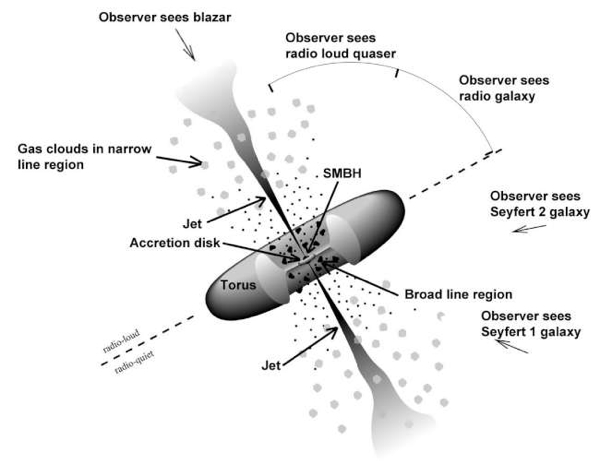
\includegraphics[width = 0.7\textwidth]{C:/Users/henri/OneDrive/Documents/NTNU/Semester 10/Masteroppgave/Plots/unified model agn.jpg}
    \caption{AGN unification}
    \label{fig:my_label}
\end{figure}

\subsection{Accretion disk}
An accretion disk is a natural consequence of the conservation of angular momentum. In the case of infalling 
matter coming close to a supermassive black hole, the matter could have some angular momentum. With this the gas should orbit the black hole at some stable distance but, due to radiative processes, fluid viscosity, and gravitational turbulence, 
the matter will lose angular momentum and spiral inwards. The inward spiral will eventually allow the matter to fall into the black hole. 
This process of inspiral is what is called accretion and the forces acting on the matter to cause the inspiral 
will also in the same process heat it up to high energies causing it to radiate. The radiation is closely linked to the 
infalling matter that is accreted onto the black hole and one can express the total luminosity of the accretion disk as 

\begin{equation}
    L_{acc} = \eta \dot{M}c^2.
    \label{eq:accretion_luminosity}
\end{equation}

Here $\eta$ is the efficiency of the accretion process, $\dot{M}$ is the mass accretion rate and $c$ is the speed of light.

%The efficiency of the accretion disk is a function of the spin of the black hole and the radius of the innermost stable circular orbit (ISCO).
%The ISCO is a counter-intuitive term in classical mechanics but in general relativity the maximum speed of a particle 
%in addition to an energy term when calculating the orbit set bounds for how close a particle can be to 
%a black hole without spiraling in. %without going into too much detail the ISCO will be a solution of this equation based on the black holes mass and spin $a$

%\begin{equation}
%    6\frac{M}{r_{ISCO}}-8\frac{aM^(\frac{1}{2})}{r^{3/2}_{ISCO}}+3\frac{a^2}{r_{ISCO}^2} = 1.
%    \label{eq:ISCO}
%\end{equation}
%It is clear from \ref{eq:ISCO} that for a non-rotating black hole the ISCO takes the radius of $6M$, the result obtained from the calculation using the Swarzschild metric.


%The accretion disk also has a bound for its maximum luminosity. As calculated for stars the Eddington
%luminosity sets a maximum strength for the radiation pressure of the accretion disk. This is given as



%\begin{equation}
%    L_{Edd} = \frac{4\pi G M m_p c}{\sigma_T}
%    \label{eq:eddington_luminosity}
%\end{equation}

The heating of the accretion disc will lead to thermal radiation from the disc and this radiation will be
proportional to the temperature of the disc. This temperature is radially dependent and if one assumes an optically thick but geometrically thin disk also called a Shakura-Sunuaev disk
one can express the radiative surface energy flux taken from \cite{BHradiation}(p. 106) as 

\begin{equation}
    \frac{dE}{dAdt}= F_{rad}(r) = \frac{3GM\dot{M}}{8\pi r^3}\left(1-\beta\sqrt{\frac{r_{\rm ISCO}}{r}}\right)
\end{equation}

Here $\beta$ is a constant that relates the fraction of angular momentum captured by the black hole, and $r_{\rm ISCO}$ is the radius of the innermost stable circular orbit. 
The temperature of the disk lie between $10^5 - 10^2$ K with emission in the optical, UV to soft X-ray range according to \cite{scholarpedia_accretion_discs}.


\subsection{Corona and X-ray emission}
From highly varying X-ray observations of AGN, it became indicative that there was a source of X-rays located close to the black hole. 
The most contemporary idea is that a corona of energetic particles is located above the accretion disk, and through inverse Compton scattering
of the optical/UV photons that arise from the accretion disk produce the seen x-ray emission. 

Inverse Compton scattering is the process of a photon gaining energy from a nearby relativistic particle. Due to the increase in efficiency 
of up scattering a photon with an electron compared to a proton, the corona x-ray emission is thought to be dominated by electrons. The process is as follows

\begin{equation}
    e^- + \gamma \rightarrow e^- + \gamma 
\end{equation}





%\subsection{Emmision lines}
%When a particle is photionized by the continuum radiation of a source it will emit a photon when it returns to its ground state. 
%This photon will have a specific wavelength that is determined by the energy difference between the two states.
%This wavelength is called the emmision line of the particle. When looking a dynamical systems with high velocities 
%the doppler shift of these emmision lines becomes important since it will affect the observed spectra of the source.

%https://lweb.cfa.harvard.edu/~pberlind/whipple/agn.html



\subsection{Broad and narrow line region}

Broad emission lines in the case of AGN are formed from the high-density gas clouds located close to the central black hole. The 
high-density parameter is inferred from the fact that one only sees broad emission from permitted line transitions (e.g. hydrogen Lyman and Balmer,
iron, and magnesium). High densities allow for collisional de-excitation and in doing so prohibit so-called forbidden transitions.
The broadening is an indication that these gas clouds are moving at huge velocities around the massive objects. This implies that they are located close to the black hole and receive the name the broad line region

Narrow emission lines are on the other hand formed in low-density gas clouds. The low densities are inferred from the fact that one sees
both permitted and forbidden line transitions. They are narrow lines due to their velocities being substantially lower than the innermost gas clouds, and from here are thought to be located further away from the black hole, in the narrow line region. 


\subsection{Dust torus}
%https://www.sciencedirect.com/science/article/pii/S0032063315000483#:~:text=This%20model%20proposes%20that%20all,collimating%20the%20radiation%20that%20escapes

The dust torus is a structure of dust that is thought to be located quite close to the black hole (0.1 - 10 pc). The main argument for the existence of this structure is the obscuration of the central region of the AGN. This obscuration 
is part of the unification scheme of AGN and was backed by the detection of polarized broad lines in AGN with their central core obscured. This polarization is what we would expect if some dust was obscuring the central region since the only light one sees is 
the light that is scattered into the line of sight according to \cite{MASON201597}. Further, the same study on the dust torus have also says that the torus is not uniform but clumpy and quite dynamic with both in and outflows of matter depending on the state of the central engine. 





\subsection{Jets}
\label{sec:jets}

A jet is a highly collimated outflow of plasma. The origin of the plasma is thought to be the accretion disk and the hot corona above it. These regions that have a high density of charged particles will under the influence of a magnetic field be accelerated and collimated into a jet-like structure.
The energy mechanism which powers the jet is not fully understood, but the most prevalent theory is the Blandford-Znajek process. It says that the rotation of the accretion disk induces a magnetic field that will interact with a rotating black hole, effectively extracting energy from the black hole and supplying it to the jet. 
The jet structure extends far beyond the local area of the AGN maintaining a stable configuration over these distances. The classification of these jets is usually divided into two groups according to \cite{walg2013relativistic}, FRI and FRII. They are differentiated by their luminosity where FRI jets are less luminous and have a more diffuse structure while FRII jets are more luminous and have a more stable structure reaching further out.
To add to this distinction it is thought that FRII jets are a product of an efficient accretion disk while FRI jets are a product of an inefficient accretion disk. This is discussed in \cite{Wei-Hao_2003} where they show that radio quiet and Seyfert 1 galaxies have lower accretion efficiency while radio loud galaxies have higher accretion efficiency. 
Beyond the energy and their structure, the jets are also notable for their emission of non-thermal radiation such as synchrotron and inverse Compton radiation. %Lastly, due to their ability to accelerate particles they are also thought to be a possible source of UHECRs and neutrinos.







\section{Types of AGN}

Before the unification of the AGN astronomers named the puzzling objects based on their observational properties. These 
names are still used to this day and are useful since their observational properties are important parameters for further study. 
The different classifications are important in understanding which objects could have the potential to produce the different observables one 
looks for in the night sky. Therefore, it seems appropriate to
discuss some different types of AGN and their observational properties. The classification in this section is heavily based on \cite{Astrobites}.

\textbf{Type I and II AGN}:
One distinguishes type I and type II AGN based on the presence of broad emission lines. In other words, this distinction is
a matter of a visible nucleus or not. Type I refers to sources whose nucleus is exposed to the observer and whose spectrum
has both narrow and broad emission lines. Type II refers to sources whose nucleus is obscured by a torus and therefore mainly has narrow emission lines.

\textbf{Blazars}:
The most extreme class of AGN. These sources are distinguished by their relativistic jets that are pointed towards the observer. 
This jet produces both synchrotron and Inverse Compton gamma rays and are extremely variable over short timescales. The
emission is also highly polarized. Often and including in this report one divides Blazars into subgroups based on the 
emission lines. The two most common are BL Lacs and Flat spectrum radio quasars (FSRQs). The difference between the two is the
presence of broad emission lines, where BL Lacs have no broad emission lines while FSRQs do. 
In addition, the distinction comes from the type of jet structure thought to be associated with the source. FRI jets for Bl Lacs and FRII for FSRQs. 

\textbf{Radio galaxies}:
Jetted AGN that as the name suggests are very bright in the radio band. They usually refer to AGN viewed edge-on, where the
torus might block the emissions from the accretion disk. The orientation of Radio galaxies gives way to strong 
synchrotron radiation, and they are often used to study the jet structure of AGN. 

\textbf{Seyfert galaxies}:
Spiral galaxies that have a bright nucleus. They are bright in the optical band and have a smaller active region 
than radio galaxies. They are often divided into two groups Seyfert I and Seyfert II where the distinction comes from type I and II. 
The galaxies also show quite high variability indicating a small emitting region. 

\textbf{Compton thin AGN}: 
A way of distinguishing AGN that can be quite useful. These AGN have lower absorption compared to Compton-thick AGN, which allow more X-rays to escape making them easier to identify. 

\textbf{Compact symmetric objects}:Compact symmetric objects were thought to be a subclass of radio galaxies that previously were thought to be young radio galaxies, but recent studies have shown that they are a distinct class of AGN and the main topic of this thesis, more on them in section \ref{sec:CSO}.

%https://iopscience.iop.org/article/10.1086/305813/fulltext/37493.text.html#:~:text=,line%20time%20delays%2C%20or%20lags


All these different distinctions are a help in understanding what processes one might be observing. The different
dominant bands indicate different processes being in the line of sight, and by considering the modern structure of 
AGN one can then try to determine the underlying dynamics.  
